\section{Integrationsmethoden}
\subsection{Substitution}
Beispiel Integral: $\int \cos{(x^2)} \cdot x \dif x$
\begin{enumerate}
  \item Substitutionsgleichung für x: $u=g(x)$ \\
    Bsp: $u = x^2$
  \item Substitutionsgleichung für dx: $\frac{du}{dx}=g'(x) \Rightarrow \dif x = \frac{du}{g'(x)}$ \\
    Bsp: $\frac{du}{dx}=2x \Rightarrow dx = \frac{du}{2x}$
  \item Integralsubstitution: $\int f(x) \dif x = \int \varphi (u)  \dif x$ \\
    Bsp: $\int \cos{(x^2)} \cdot x  \dif x = \int \cos{(u)} \cdot x \cdot \frac{du}{2x} = \int \frac{1}{2} \cos{(u)} \dif u$
  \item Integration: $\int \varphi(u) \dif u = \Phi(u) + C$ \\
    Bsp: $\int \frac{1}{2} \cos{(u)} \dif u = \frac{1}{2} \int \cos{(u)} \dif u = \frac{1}{2} \sin{(u)} + C$
  \item Rücksubstitution (Bei unbestimmten Integralen) \\
    Bsp: $\frac{1}{2} \sin(u) + C = \frac{1}{2} \sin{x^2} + C$
\end{enumerate}

\subsubsection{Substitution Speziallfall}%
\label{ssub:Substitution Speziallfall}
Ist die Funktion $u(x)$ linear, so lässt sich das Integral mit Hilfe einer Abkürzung bestimmen. Für eine Funktion $f$ und Konstanten $a, b$ gilt:
\begin{equation*}
  \int f(ax + b) \dif x = \frac{1}{a} \cdot F(ax + b)
\end{equation*}

\subsection{Partielle Integration}
\begin{equation*}
  \int u(x) \cdot v'(x) \dif x = u(x) \cdot v(x) - \int u'(x) \cdot v(x) \dif x
\end{equation*}
\begin{equation*}
  \int_{a}^{b} u(x) \cdot v'(x) \dif x = \left[ u(x) \cdot v(x) \right]^b_a - \int_{a}^{b} u'(x) \cdot v(x) \dif x
\end{equation*}

\begin{center}
  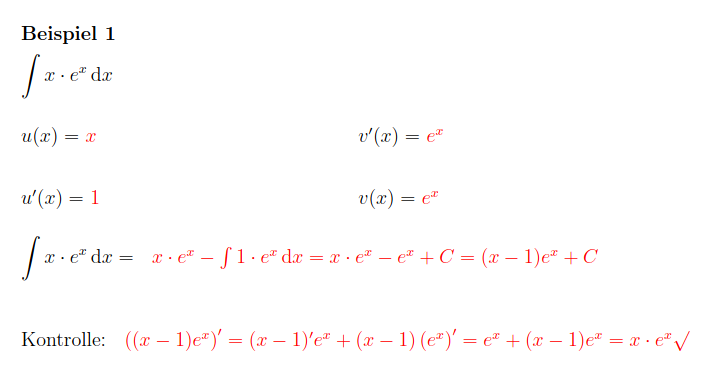
\includegraphics[width=0.9\linewidth]{images/partiell1.png}
  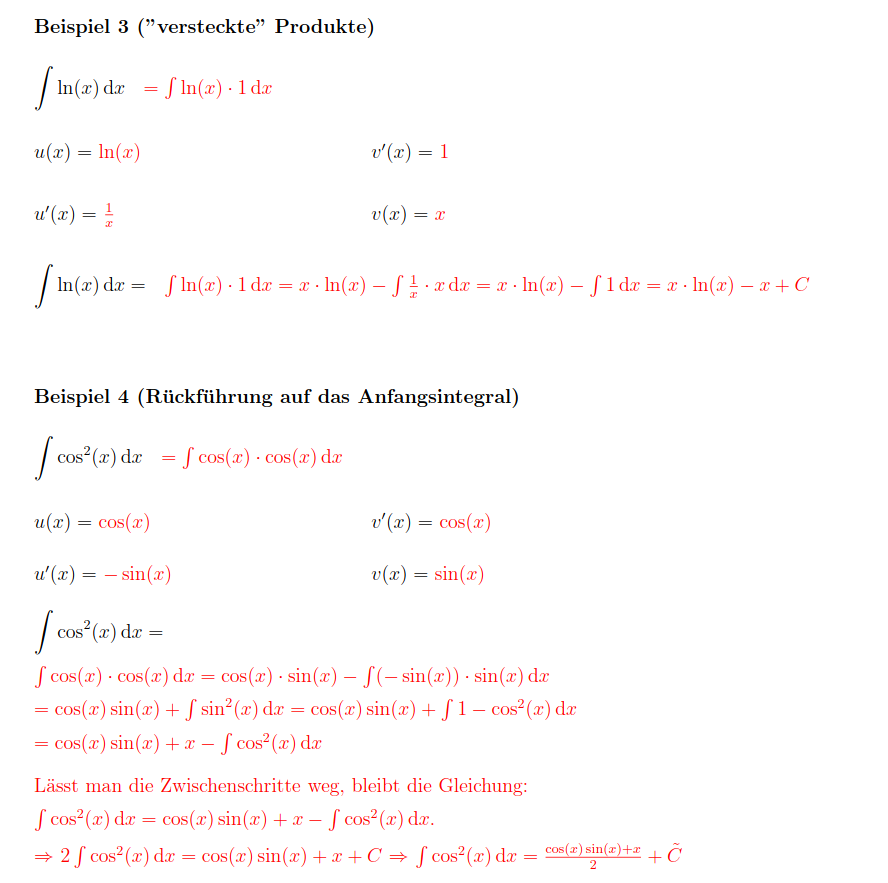
\includegraphics[width=0.9\linewidth]{images/partiell2.png}
\end{center}

\subsection{Partialbruchzerlegung}
Achtung: Bei unecht gebrochenrationalen Funktionen zuerst mit Polynomdivision umformen! \\
Beispiel Integral: $f(x) = \frac{x + 1}{x^3 - 5x^2 + 8x -4}$
\begin{enumerate}
  \item Nullstellen des Nenners h(x) mit Multiplizitäten bestimmen: 
    \begin{enumerate}
      \item Bsp: Erraten: $x_1 = 1$
      \item Linearfaktor abspalten mithilfe des Hornerschemas
      \item Verbleibendes Polynom: $p(x) = x^2 -4x + 4 = (x-2)^2$
    \end{enumerate}
  \item Jeder dieser Nullstellen wird eine Summe von Brüchen zugeordnet: \\
    $x_1$ ist einfache Nullstelle $\rightarrow \frac{A}{x - x_1}$ \\
    $x_1$ ist $n$-fache Nullstelle $\rightarrow \frac{A_1}{x - x_1} + \dots + \frac{A_n}{(x-x_1)^n}$ \\
    Bsp: $x_1 \rightarrow \frac{A}{x-1} \quad x_2 \rightarrow \frac{B}{x-2} + \frac{C}{(x-2)^2}$
  \item f(x) wird mit der Summe aller Partialbrüche gleichgesetzt: \\
    Bsp: $f(x) = \frac{x+1}{x^3 - 5x^2 + 8x -4} = \frac{A}{x - x_1} + \frac{A_1}{x - x_1} + \dots + \frac{A_n}{(x-x_1)^n}$
  \item Bestimmung der Konstanten
    \begin{enumerate}
      \item Alle Partialbrüche auf einen gemeinsamen Nenner bringen \\
        Bsp: $\frac{A(x-2)^2 + B(x-1)(x-2) + C(x-1)}{(x-1)(x-2)^2}$
      \item Durch einsetzen von $x$-Werten erhält man ein lineares Gleichungssystem \\
        Bsp: $x = 1 \rightarrow 2 = A$ etc.
      \item Gleichungssystem lösen
    \end{enumerate}
\end{enumerate}

\subsubsection{Integration der Partialbrüche}%
\label{ssub:Integration der Partialbrüche}
\begin{equation*}
  \int \frac{1}{x-x_0} \dif x = \int \frac{1}{u} \dif u = \ln |u| + C = \ln |x-x_0| + C
\end{equation*}
\begin{align*}
  \int \frac{1}{(x-x_0} \dif x = \int \frac{1}{u^-r} \dif u = \frac{u^{-r+1}}{-r + 1} + C = \frac{(x-x_0)^{-r+1}}{1-r}+C \\ 
  = \frac{1}{(1-r)(x-x_0)^{r-1}}+C
\end{align*}

\subsection{Muster für die jeweiligen Integrationsmethoden}

\begin{center}
  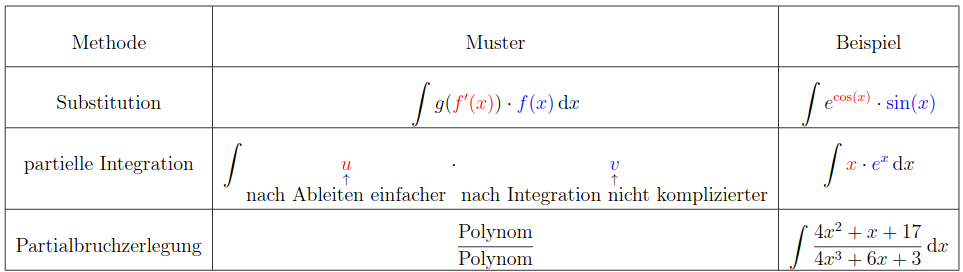
\includegraphics[width=0.9\linewidth]{images/muster.png}
\end{center}
